\documentclass[10pt]{article}
\usepackage[a4paper,left=2.54cm,top=2.54cm,right=2.54cm,bottom=2.54cm]{geometry}
\usepackage{fancyhdr}
\setlength{\headsep}{1.cm} % Adjust the space after the header
\usepackage{afterpage}
\usepackage{setspace}
\usepackage{bibspacing}
\usepackage{float}
\singlespacing

%%%% YOU CAN PUT YOUR OWN DEFINITIONS HERE
\newfont{\toto}{msbm10 at 12 pt}
\newfont{\ithd}{cmr9}
\newcommand{\equa}[1]{(\ref{eq:#1})}
\newcommand{\laeq}[1]{\label{eq:#1}}
\newcommand{\figu}[1]{\ref{fig:#1}} 
\newcommand{\lafi}[1]{\label{fig:#1}}
\newcommand{\fmo}{\tilde{U}}
\newcommand{\fve}{\tilde{u}}
\newcommand{\Dt}{\Delta t}

\newcommand{\R}{\mathbb{R}}
\newcommand{\Z}{\mathbb{Z}}
\newcommand{\si}[1]{\rm\scriptscriptstyle{#1}}
%%%% END OF YOUR DEFINITIONS 

\pagestyle{fancyplain}
\renewcommand{\headrulewidth}{0pt}

\usepackage{amsmath,amsthm,amsfonts,amssymb}
\usepackage{physics}
\usepackage[pdftex]{graphicx}
\usepackage[T1]{fontenc}

%%%% CONFERENCE HEADER. REPLACE xxxx WITH 4-DIGIT PAPER NUMBER ASSIGNED BY CONFERENCE COMMITTEE.

\rhead{\ithd{\bf ICCFD12-2024-xxxx\\  \   \\}}
\lhead{\ithd{\bf Twelfth International Conference on \\      
Computational Fluid Dynamics (ICCFD12), \\
Kobe, Japan, July 14-19, 2024
}}


\usepackage{titling}
\setlength{\droptitle}{0em}  
\pretitle{\vspace{-4em}\begin{center}\LARGE}
\posttitle{\end{center}\vspace{-1em}}
\preauthor{\begin{center}\large}
\postauthor{\end{center}\vspace{-6em}}


\title{
\bf A Novel Energy-based Artificial Viscosity for Suppressing Numerical Oscillations in Discontinuous Gakerlin and Flux Reconstruction Schemes
}
\author{
Weicheng Pei$^{*}$ and Yu-Xin Ren$^{*}$\\
Corresponding author: weicheng.pei@icloud.com\\
$^{*}$ Department of Engineering Mechanics, Tsinghua University, Beijing 100084, China
}
\date{}

\begin{document}

%%%% TITLE
\maketitle
\afterpage{\fancyhead{}}

%%%% ABSTRACT AND KEYWORDS
%\vskip0.5cm
\centerline{
}
\vskip0.5cm 

%%%% MAIN PART
\section{Introduction}
To construct high-order schemes on unstructured meshes, the discontinuous Gakerlin (DG) method \cite{Cockburn_2001} and the flux reconstruction (FR) method \cite{Huynh_2014} are two of the most popular choices in the community of computational fluid dynamics (CFD).
%
Besides the inherent compactness, these schemes are much easier to implement $p$-refinement than their finite difference and finite volume counterparts.
%
However, like other high-order schemes, numerical oscillations would appear near discontinuities or large gradients in the solution given by a DG or FR scheme, if no shock capturing mechanism were incorporated into it.

In this paper, a novel artificial viscosity based on an energy measure of oscillation and its damping rate on a DG or FR element is developed.
%
The oscillation energy, which measures the amplitude of numerical oscillations on a given element, is obtained by evaluating the $L_2$-norm of the difference between the numerical solutions on the element and its neighbors.
%
The damping rate of this energy on an element can be derived under the assumptions of linear flux--gradient relation and constant viscosity distribution.
%
The value of viscosity for suppressing numerical oscillations is obtained by taking the ratio of the oscillation energy with respect to the product of its damping rate and prescribed time step.
%
Such element-wise constant viscosity distribution is reconstructed to be $C_0$ constinuous on element interfaces.

Standard cases for testing shock capturing schemes show that the proposed mechanism is sufficiently large for suppressing numerical oscillations near physical discontinuities, such as shocks and contacts, while keeps negligible in other regions for maintaing the high-orderness of the DG or FR solution.

\section{Problem Statement}
\subsection{DG and FR Schemes}
To obtain an element-wise $p$-degree polynomial approximation of the solution of the 1D conservation law
$$
\pdv{u}{t}+\pdv{f(u)}{x}=0,
$$
one may first introduce a Lagrange interpolation for both $u$ and $f$ on the $j$th element:
$$
u^h_j(x,t) = \sum_{k=0}^{p} L_{j,k}(x)\,\hat{u}_{j,k}(t),\quad
f^h_j(x,t) = \sum_{k=0}^{p} L_{j,k}(x)\,f(\hat{u}_{j,k}(t)),
$$
in which $L_{j,k}$ is the Lagrange basis associated with the $k$th node (a.k.a. solution point) on the $j$th element, and $\hat{u}_{j,k}$ is the value of the approximate solution $u^h$ on that node.
An ordinary differential equation (ODE) system can then be derived from either the DG method or the FR method.

\subsection{Oscillation Energy}
To measure the numerical oscillations quantitatively, we define the oscillation energy on the $j$th element to be
$$
\Delta K_j = \int_{x_{j-1/2}}^{x_{j}}\left(u_{j}^{h}-u_{j-1}^{h}\right)^{2}\dd{x}+\int_{x_{j}}^{x_{j+1/2}}\left(u_{j}^{h}-u_{j+1}^{h}\right)^{2}\dd{x},
$$
which is the square of the $L_2$-norm of difference between the solution on $E_j$ and those on its immediate neighbors.
The integrals are as cheap as weighted summations of nodal values if solution points are also Gaussian quadrature points, which is a common practice in the DG spectral element method (SEM) \cite{Li_2020}.

\subsection{Artificial Viscosity}
To dissipate the oscillation energy just defined, we introduce an artificial viscosity term, which is linear to the gradient of solution, to the conservation law, which becomes
$$
\pdv{u}{t}+\pdv{f(u)}{x}=\pdv{x}\qty(\nu\pdv{u}{x}),\quad \nu >= 0.
$$
The ODE system given by the DG or FR scheme becomes
$$
\dv{t}\ket{\hat{u}_{j}}=\cdots+\nu_{j}\left(\underline{D}_{j}\ket{\hat{u}_{j}}+\underline{E}_{j}\ket{\hat{u}_{j-1}}+\underline{F}_{j}\ket{\hat{u}_{j+1}}\right),
$$
where $\ket{\hat{u}_{j}}, \ket{\hat{u}_{j-1}}, \ket{\hat{u}_{j+1}}$ are column matrices formed by nodal values on $E_{j}, E_{j-1}, E_{j+1}$ respectively, and $ \underline{D}_{j}, \underline{E}_{j}, \underline{F}_{j} $ are constant square matrices given the spatial discretization and the numerical flux on element interfaces.
The dissipattion rate of the kinetic energy is
$$
\dv{t}\underbrace{\frac{1}{2}\Vert u_{j}^{h}\Vert_{L_{2}(E_{j})}^{2}}_{K_{j}}=\bra{\hat{u}_{j}}\underline{W}_{j}\dv{t}\ket{\hat{u}_{j}}=\cdots+\nu_{j}\,\underbrace{\left(\bra{\hat{u}_{j}}\underline{W}_{j}\,\underline{D}_{j}\ket{\hat{u}_{j}}+\cdots\right)}_{G_{j}},
$$
where $\underline{W}_{j}$ is the diagonal matrix form by Gaussian quadrature weights.
The value of viscosity is given by
$$
\nu_{j}=\frac{\Delta K_{j}}{-G_{j}\,\tau}\impliedby\dv{t}K_{j}=\cdots+\nu_{j}\,G_{j},
$$
which means the oscillation energy $\Delta K_{j}$ is dissipated by the viscosity within a prescribed length of time $\tau$.

\section{Results}
In this section, the effectiveness of the artificial viscosity proposed in the previous section is demonstrated by some standard test cases.
The computational domain is divide into $100$ elements uniformly.
A fifth-order ($p=4$) FR scheme using the $g_2$ correction function, which is equivalent to a DGSEM scheme of the same order of accuracy, is used for spatial discretization.
The resulting ODE system is solved by an explicit three-stage third-order strong stability preserving Runge--Kutta method.

\subsection{Shock Tube Problems}
Riemann problems, as well as their exact and approximate solvers, play a pivot role in the development of CFD schemes \cite{Toro_2009}.
Among the infinite number of Riemann problems of the 1D Euler system, the Sod problem with the initial condition
\begin{equation}
\mqty[\rho & u & p]_{t=0}
=
\begin{cases}
\mqty[1 & 0 & 1], &x<0,\\
\mqty[0.125 & 0 & 0.1], &x>0,\\
\end{cases}
\end{equation}
and the Lax problem in with the initial condition
\begin{equation}
\mqty[\rho & u & p]_{t=0}
=
\begin{cases}
\mqty[0.445 & 0.698 & 3.528], &x<0,\\
\mqty[0.5 & 0 & 0.571], &x>0,\\
\end{cases}
\end{equation}
are two of the most famous ones that are frequently used for testing shock capturing mechanisms.

Figure \ref{fig:sod} and \ref{fig:lax} gives the solution (the "Actual" curves) of these two problems at the moment ($t=0.5$ for Sod, $t=0.3$ for Lax) and the viscosity distributions for each characteristic variables at all time steps.
The "Expect" curves in these figures are the exact solutions obtained from analytical procedures.
\begin{figure}[H]
  \centering
  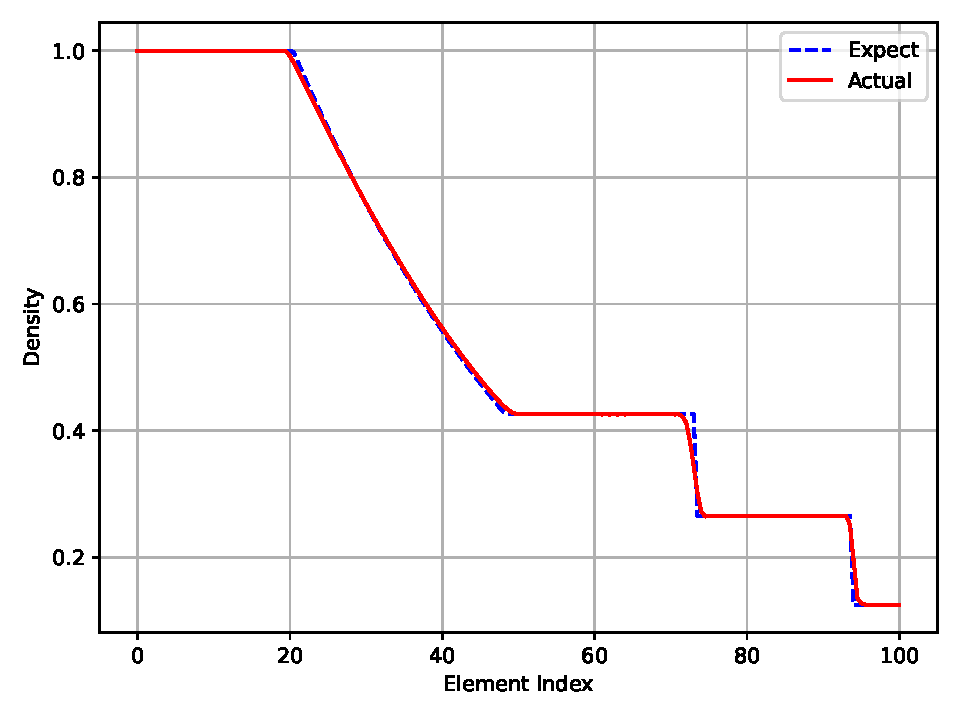
\includegraphics[width=.49\textwidth]{./sod/Frame100.pdf}
  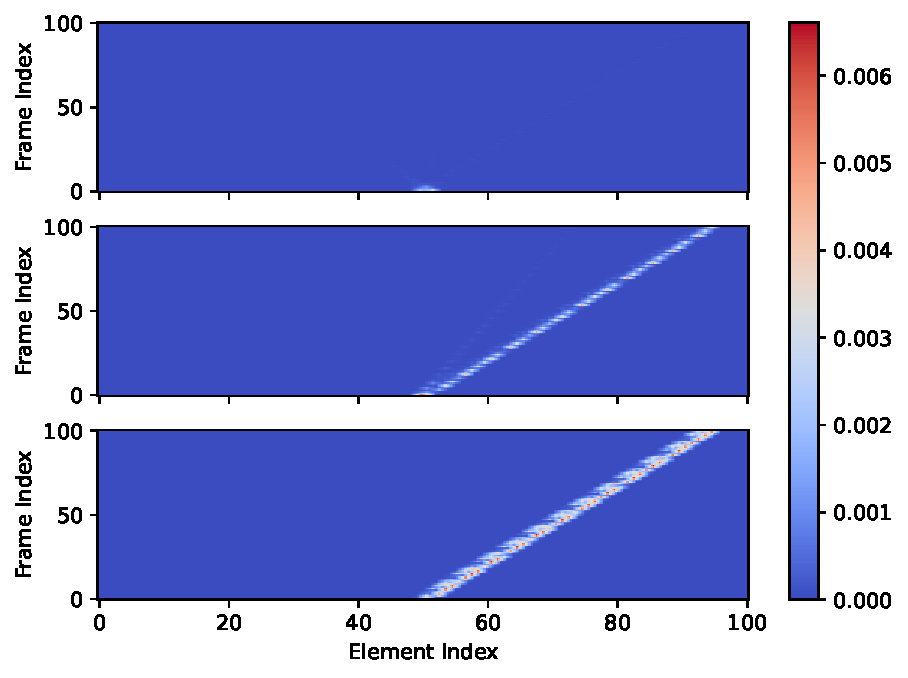
\includegraphics[width=.49\textwidth]{./sod/Viscosity.pdf}
  \caption{Solution and viscosity distribution of the Sod problem.}
  \label{fig:sod}
\end{figure}

\begin{figure}[H]
  \centering
  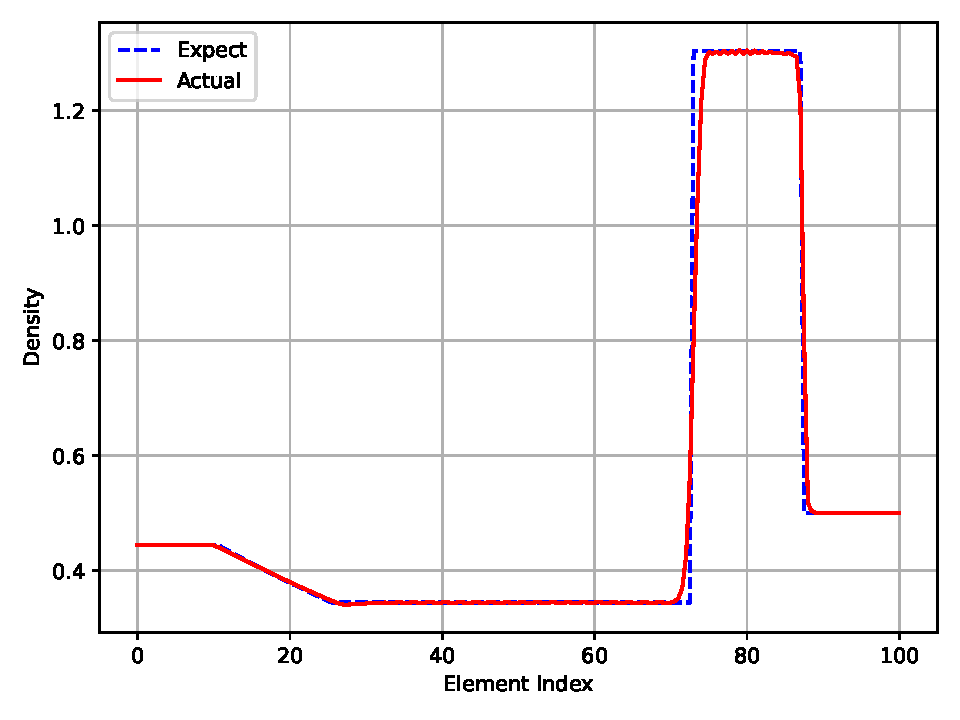
\includegraphics[width=.49\textwidth]{./lax/Frame100.pdf}
  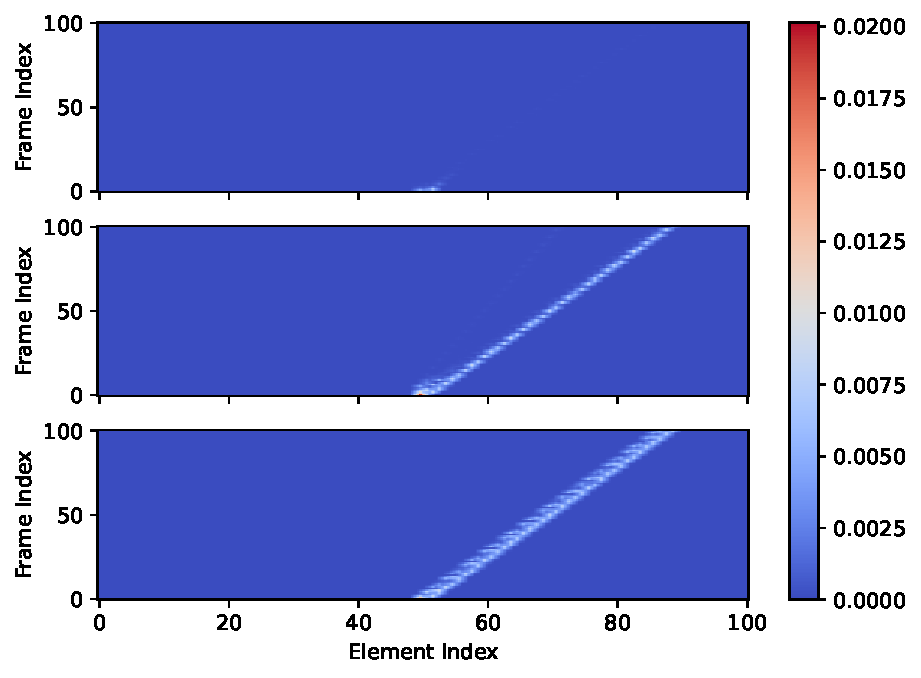
\includegraphics[width=.49\textwidth]{./lax/Viscosity.pdf}
  \caption{Solution and viscosity distribution of the Lax problem.}
  \label{fig:lax}
\end{figure}

\subsection{The Shu--Osher Problem}\label{sec:shu_osher}
This problem is designed to mimic the interaction of a running shock with a standing isentropic wave \cite{Shu_1989}.
The computational domain is $x\in[0, 10]$ with two no-reflection conditions applied at the left and right boundaries.
The time range of interest is $t\in[0, 1.8]$ with the initial condition set to be
\begin{equation}
\mqty[\rho & u & p]_{t=0}
=
\begin{cases}
\mqty[3.857143 & 2.629369 & 10.33333], &x\in[0,1);\\
\mqty[1+0.2\sin(5x) & 0 & 1], &x\in(1,10].
\end{cases}
\end{equation}

Figure \ref{fig:shu_osher} gives the solution (the "Actual" curve) of this problem at the final ($t=1.8$) moment and the viscosity distribution for each characteristic variables at all time steps.
The "Expect" curve in this figure is the approximate solution given by the same FR scheme with a $p$-weighted limiter \cite{Li_2020} on a finer mesh (200 elements).
\begin{figure}[H]
  \centering
  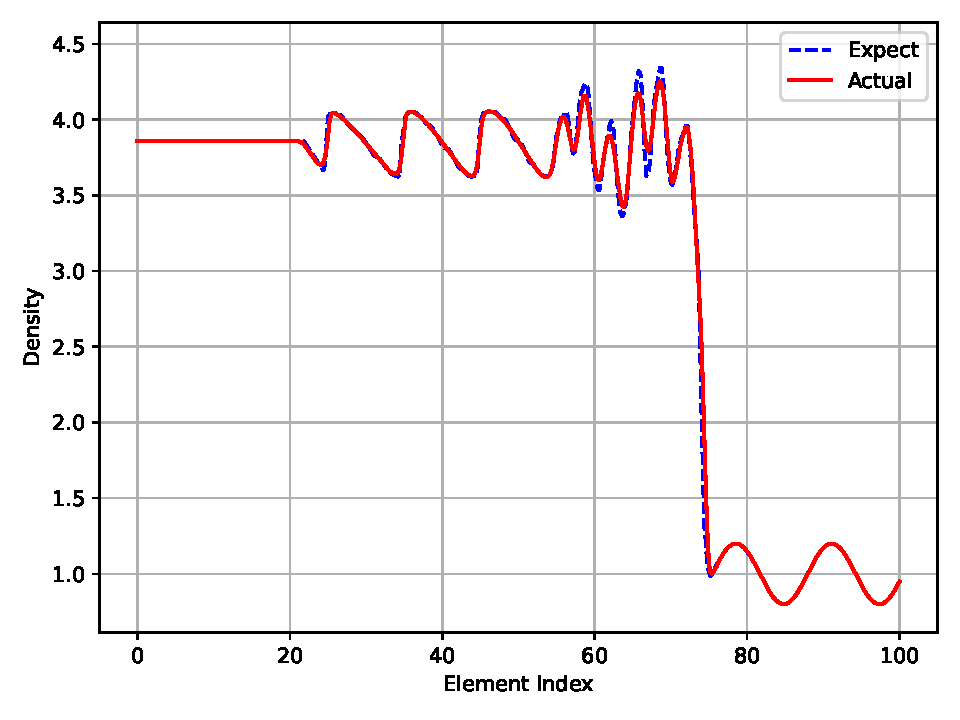
\includegraphics[width=.49\textwidth]{./shu_osher/final/Frame100.pdf}
  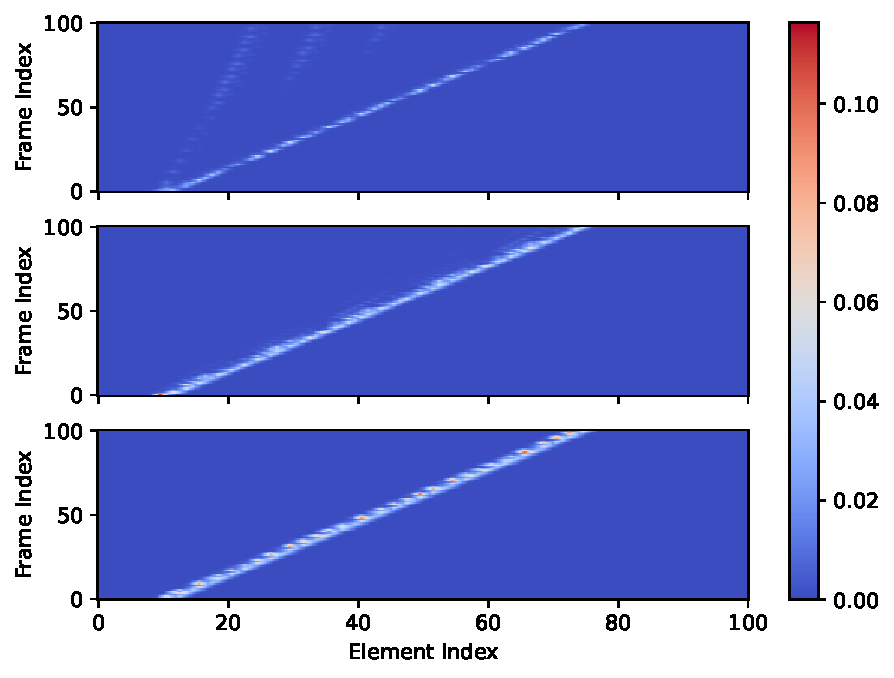
\includegraphics[width=.49\textwidth]{./shu_osher/final/Viscosity.pdf}
  \caption{Solution and viscosity distribution of the Shu--Osher problem.}
  \label{fig:shu_osher}
\end{figure}

%%%% BIBLIOGRAPHY
\bibspacing=\dimen 100
\bibliographystyle{unsrt}
\bibliography{biblio}

\end{document}
